\chapter{Konzeption}

In diesem Kapitel wird die Konzeption dieses Projektes von zwei Aspekten erzählt, nämlich Learning Managment System (LMS) und WebVR, Vorbereitung einer Infusion mit Web VR.

Bei Learning Managment System (LMS) und WebVR wird erst die Konzeption eines Unterrichts auf LMS beschreibt. VR-Training wird als eine Lernmethode in diesem Unterricht eingefügt.

Um die geeigneter VR Technik mit LMS zu verbeinden, werden native VR Applikations mit Web VR Applikations vergleicht. Auf dem Ergebnis des Vergleichs wird Web VR Technik entschieden.

Die Web VR Applikation kann in drei Formen mit LMS verbinden. Die drei Formen werden mit einander vergleicht. Und eine davon wird in diesem Projekt eingesetzt.

Bei Vorbereitung einer Infusion mit Web VR werden die Web VR Applikation von drei Aspekten vorgestellt, Graphical user interface (GUI), Interaktion, und Anordnung. Dadurch werden die sechs Kategorien der Immersion konkretisiert.

Graphical user interface (GUI) beschreibt die simulierte VR Umgebung. Das ist die Grundlage, dass die praktische Übung ohne reale Materialien zu machen.

Interaktion beschreibt, wie der Benutzer die virtuelle Welt beeinflussen. Da ist ein Ziel des Projektes, cross-platform zu sein, wird die Interaktionen durch unterschiedlichen Geräte beschreibt.

Als eine Übung müssen die richtige und fachliche Handlungen vermittelt, deswegen werden die Aktionen des Benutzers kontrolliert und geleitet. Bei Anordnung werden die Methoden, eine effektive Übung reibungslos durchzuführen. 

\section{Learning Managment System (LMS) und WebVR}
Laut der Forschung entscheidet die Lernmethode für den Lerneffekt. WevVR Technik bietet die neue Möglichkeit, neue Lernmethode beispielsweise VR-Training zu entwickeln. Hier wird eine Konzeption eines mit VR-Training verbundenen Unterrichts auf LMS erzählt.

 \subsection{Erstellung eines Unterrichts}
 Die VR Übung ist eine ergänzige Lernmethode für das Lernen. Vor der Durchführung der Übung sollen genügendes Vorwissen angeboten werden. Deswegen wird erst einen Unterricht auf Learning Managment System erstellt.

 Laut der Erklärung im Kapitel Stand der Forschung \glqq Multisensorische und emotionale Wahrnehmungen können die Gedächtnisleitung verstärken\grqq\ sollen die Lernmaterialien des Unterrichts vielfältig sein.  Durch drei Lernmateriallien werden das Vorwissen geboten:
 \begin{enumerate}
    \item Text: Text ist das traditionelle Lernmaterial. Es spielt eine unersetzbare Rolle für Lernen. Die Lesegeschwindigkeit kann der Lernende sich selbst entscheiden. Während des Lesens kann der Leser gut denken, merken und notieren.
    \item Video: Video ist ein intuitives Lernmaterial. Zwei Wahrnehmungen, Sehen und Hören werden aufgerufen, wenn man Video anschaut. Durch Video kann die Handlung sehr konkret gezeigt. Zur Zeit ist Video das beste und verbreitete Medium, praktische Kenntnisse zu vermitteln.
    \item Diagramm: Diagramm ist eine optimale Darstellung für Struktur und Sequenz. Die deutliche visuelle Zeichnungen sind hilfreich für das Verständnis und Gedächtnis.
 \end{enumerate}

 Nach der Sammlung der Vorkenntnisse geht der Lernende durch die Zugang in diesem Unterricht in VR Umgebung rein, und wird die praktische Übung durchgeführt. In der Übung steht das Vorwissen als Hinweise zu Verfügung. Die Hinweise müssen nicht zwingend angeschaut werden, wenn der Lernende die Übung flüssig schaffen kann. Allerdings soll die Hinweise einfach erreichbar sein. Sodass muss der Lernende nicht aus VR Umgebung ausgehen, um Hilfsmittel zu suchen, wenn der Lernende nicht an der Vorkenntnisse erinnern kann. Wenn die Übung geschafft wird, wird der Lernende wieder zu dem Unterricht geleitet.

 Nach der Übung wird ein Test geboten, um das Ergebnis des Lernens zu prüfen. Das Ergebnis des Tests wird in Learning Managment System gespeichert und als Feedback an dem Lehrende geschickt.

 \subsection{WebVR}
 Zwei Ziele des Projekts haben höchste Prioritäten: gute Erreichbarkeit und Verbindung mit LMS.

 Der größte Vorteil der native Apps bei Erreichbarkeit ist offline Benutzbarkeit. Wenn die Applikation installiert ist, muss es während der VR Übung nicht online sein. Allerdings die Installation besitzt viele Kapazität von Rechner oder Smartphone. Wenn viele Übungen werden in eine Applikation eingepackt, führt es zu Missbrauch der Kapazität, weil tatsächlich die geschaffte Übungen nicht gebraucht sind. Wenn jede Übung eigne Applikation hat, wird viele extra Zeit in Installation vor dem Lernen investiert, sodass existiert der Vorteil offline Erreichbarkeit nicht mehr.

 Capterra ist eine Webseite, die deren Benutzer hilft, geeignet Software in unterschiedlichen Bereichen zu finden. Es werden insgesamt 432 Softwares gefunden, wenn \glqq LMS Software \grqq\ gesucht wird. 406 von 432 gefundene LMSs haben web basierte Applikation zu Verfügung. Das heißt, dass 94\% LMS können in Browser laufen lassen.

 WebVR Applikation wird auch in Browser aufgerufen. Ohne software Wechseln wird zu keiner Ablenkung geführt. Außerdem ist die Schnittstelle zwischen Web Applikationen einfach zu implementieren. Darüber hinaus fordert LMS sowieso Internet, kann die Anforderung für Internet von WebVR nicht als Nachteil gelten. 

 Laut oben genannten Gründe wird für WebVR Technik entschieden, die VR Übung zu realisieren.

 \subsection{Verbindung zwischen WebVR Applikation und Learning Managment System}
 Es gibt drei Formen für die Verbindung zwischen WebVR Applikation und Learning Managment System(LMS):
 \begin{enumerate}
   \item WebVR Applikation neben dem Learning Managment System:
     \subitem In LMS wird die Zugang zur VR Umgebung geboten und durch URL können Informationen in VR Umgebung eingefügt werden. In Vr Umgebung wird auch die Zugang zurück zu LMS geboten. Aber keine Information kann von VR Umgebung an LMS übermittelt werden.
     
     Der Vorteil ist, dass die WebVR Applikation unabhängig von LMS ist. Jede LMS kann mit der WebVR Applikation verbinden.
     
     Der Nachteil ist, dass der Umtausch der Informationen ziwischen WebVR Applikation und LMS einspurig ist. Das LMS kann Keine Information von WebVR Appliaktion bekommen. Außerdem wird jede Änderung in WebApp z.B. Umschreibung des Hinweises durch Programmierer gemacht. Der Lehrende ist nicht in der Lage, alleine die Übung zu verbessern oder korrigieren.
     
   \item WebVR Applikation teilweise in dem Learning Managment System:
     \subitem In LMS wird die Zugang zur VR Umgebung geboten, allerdings die Zugang nicht ein URL, sondern erfahrungsmäßig ein Plugin ist. Durch das Plugin kann die WebVR Applikation die versteckte zugängliche Daten der Datenbank des Unterrichts bekommen. Mit solche Daten ist die WebVR Applikation in der Lage, die Daten in Datenbank zu speichern und die Daten aus Datenbank zu lesen. Durch das Middleware wird die gegenseitige Kommunikation zwischen WebVR Applikation und LMS ermöglichen. Obwohl durch URL die zugängliche Daten auch übergetragen werden können, ist es sehr unsicher für das LMS.
     
     Der Vorteil ist, dass die Kommunikation zwischen WebVR Applikation und LMS frei ist. Das heißt, dass die übergetragene Daten nicht nur Parameter sondern auch Bilder, Audios und Videos sein können und das LMS kann die Informationen, die während der Übung in WebVR Applikation erstellt, bekommen. Darüber hinaus kann der Lehrende durch dem Plugin die Inhälte in WebVR Applikation direkt andern.
     
     Die Nachteile sind, dass die WebVR Applikation von dem LMS abhängig ist und die Entwicklung aufwendig ist. Um die Daten barrierefrei überzutragen, muss entsprechende Schnittstelle in WebVR Applikation konfiguriert werden. Bei der Entwicklung werden nicht nur WebVR Applikation, sondern auch das Plugin von LMS geschrieben. Zusätzlich wird eine Datenbank eingerichtet.
     
   \item Learning Management System in WebVR Applikation
     \subitem Bei dieser Form ist die Methode der Kommunikation zwischen WebVR Applikation und LMS gleich wie die zweite Form. Der größte Unterschied liegt an der Benutzererfahrung. Die Graphical User Interface(GUI) des LMSs wird in der VR Umgebung dargestellt. Das heißt, dass vom Anfang an der Lernende in der VR Umgebung steht. In der VR Umgebung wird Vorwissen gesammelt, praktische Übung durchgeführt und Test gemacht.
     
     Der Vorteil ist, dass der ganze Lernprozess in VR Umgebung integriert wird, keine Ablenkung existiert.
     
     Die Nachteile sind aufwendige Entwicklung und ungewöhnliche Erfahrung des Lesens.
 \end{enumerate}
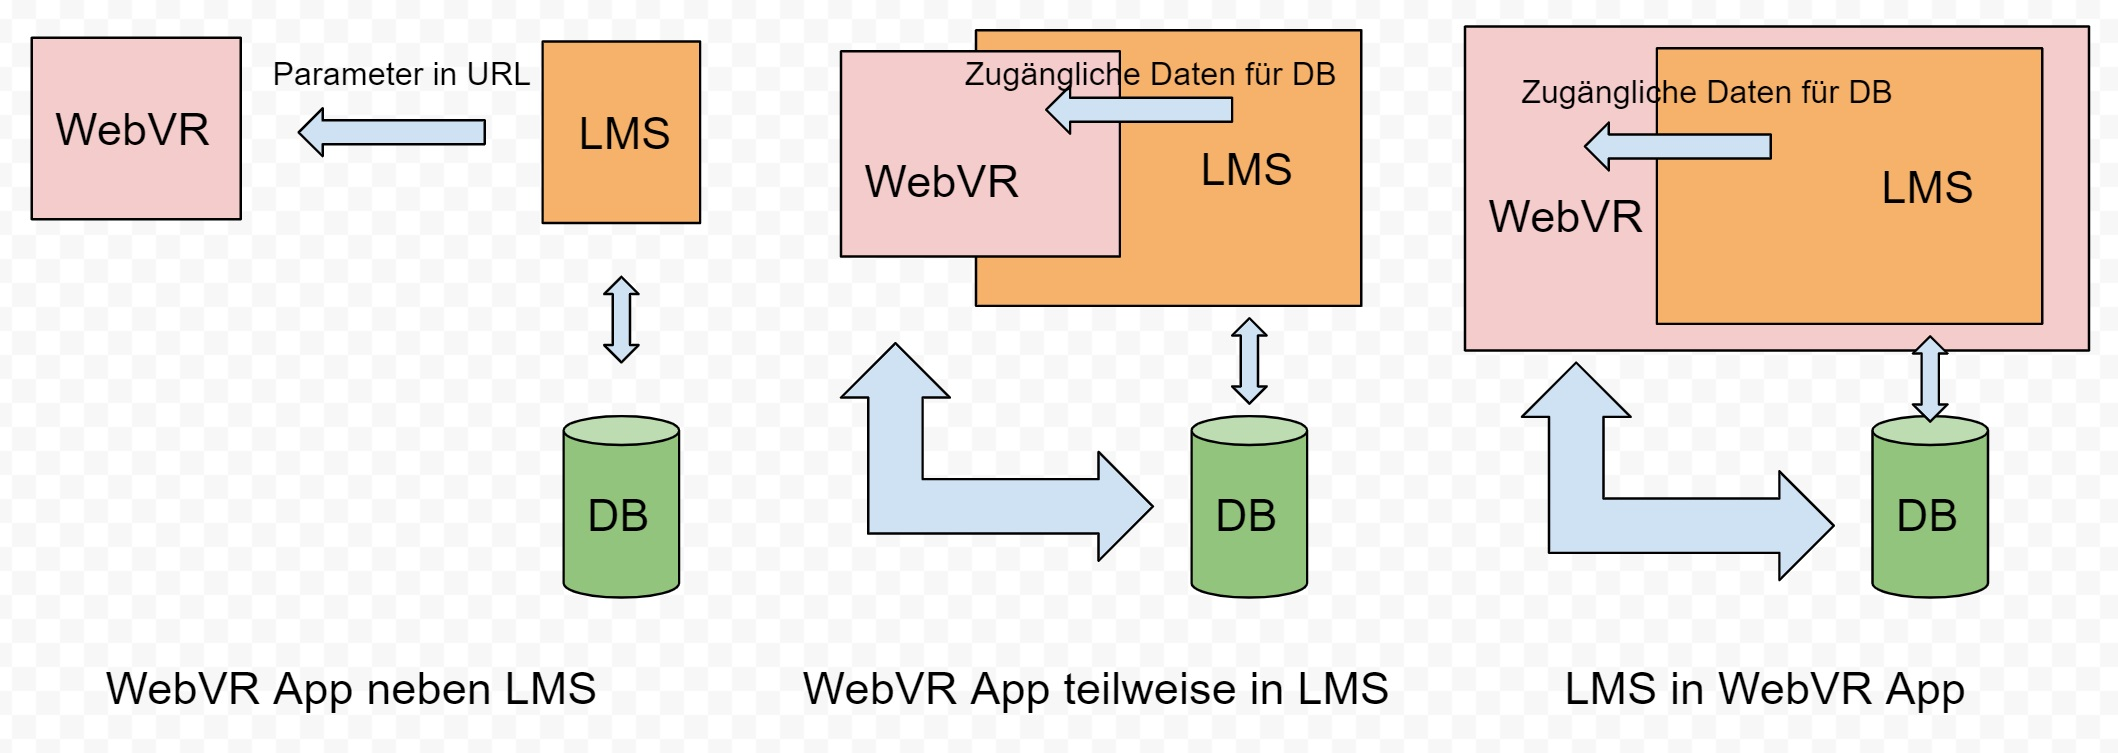
\includegraphics[width=\textwidth]{images/formenDerVerbindung.jpg}

Bei diesem Projekt wird erste Form implementiert. Wegen der begrenzte Entwicklungszeit werden die zweite und dritte Formen bei diesem Projekt nicht realisiert.

\section{Vorbereitung einer Infusion mit WebVR}

Als der Schwerpunkt des Projektes wird die Konzeption der Übung Vorbereitung einer Infusion mit WebVR ausführlich erklärt. Die Konzeption wird nach der Kategorien der Immersion von Jason Jerald\citep{28} aufgebaut.

 \subsection{Graphical user interface (GUI)}
 GUI ist die visuelle Darstellung eine Applikation. Für dieses Projekt ist GUI die simuliert Umgebung. Laut der Forschung führt lebendiger Simulation zu bessere Gedächtnis bei VR-Training. Die Kategorien Extensiveness, Surroundness und Vividness wurden durch der GUI realisiert.
 
  \subsubsection{Szene}
  Die VR Umgebung bezieht sich auf dem \glqq Skillslab\grqq\ in Fachhochschule Bielefeld. Um der relevante Objekte der Übung zu betonen, wird die Szene vereinfacht.
  
  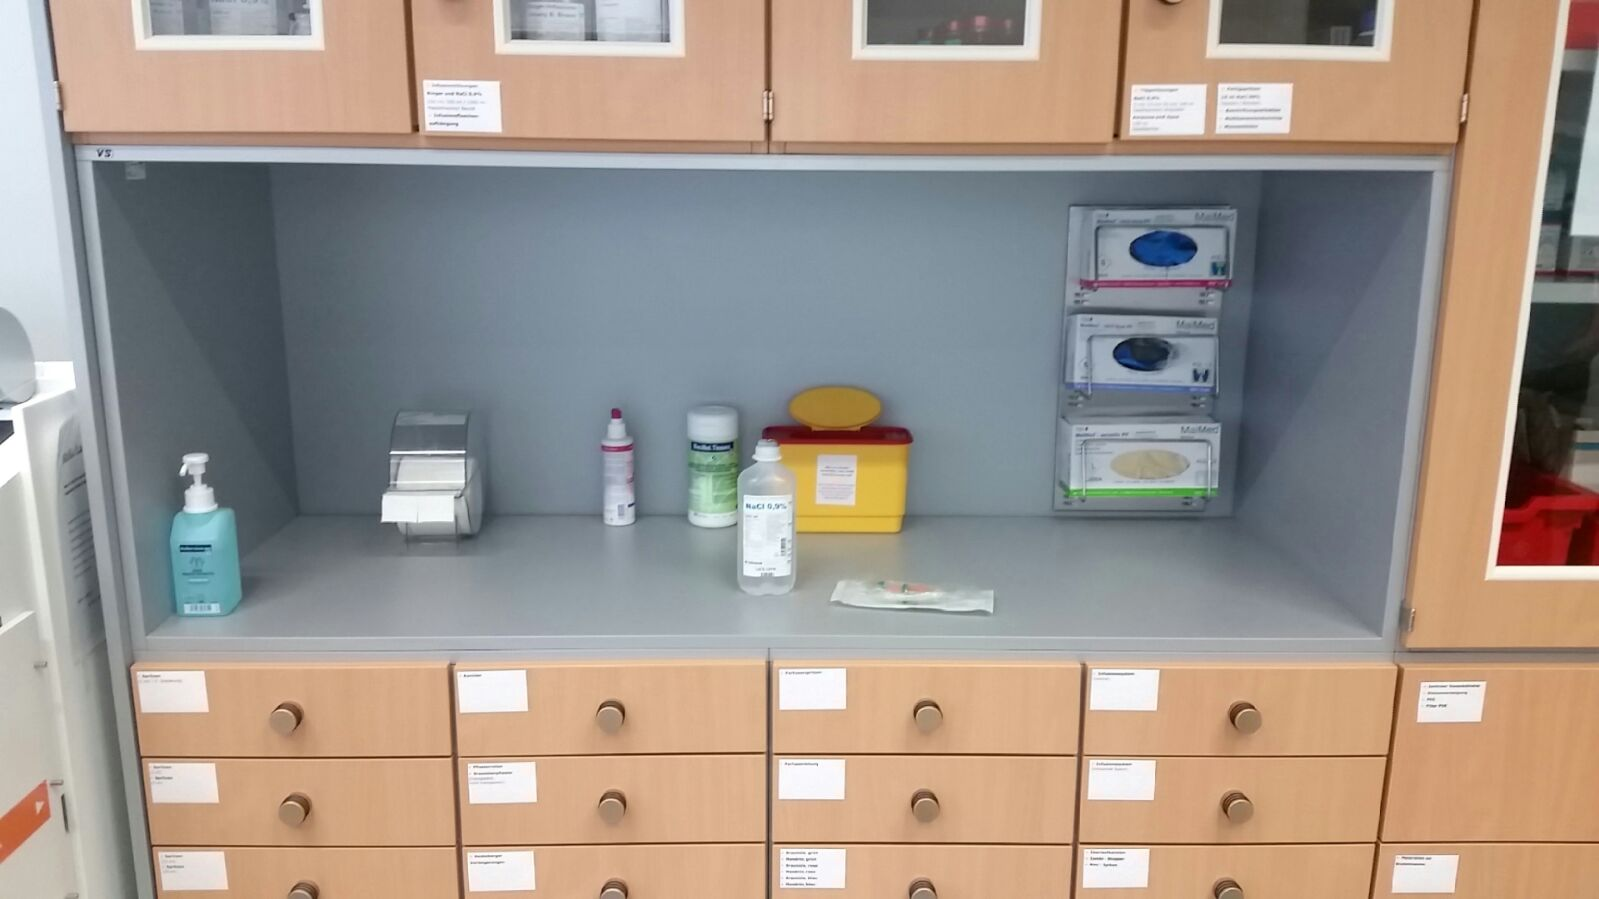
\includegraphics[width=\textwidth]{images/RealLabor.jpg}
  
  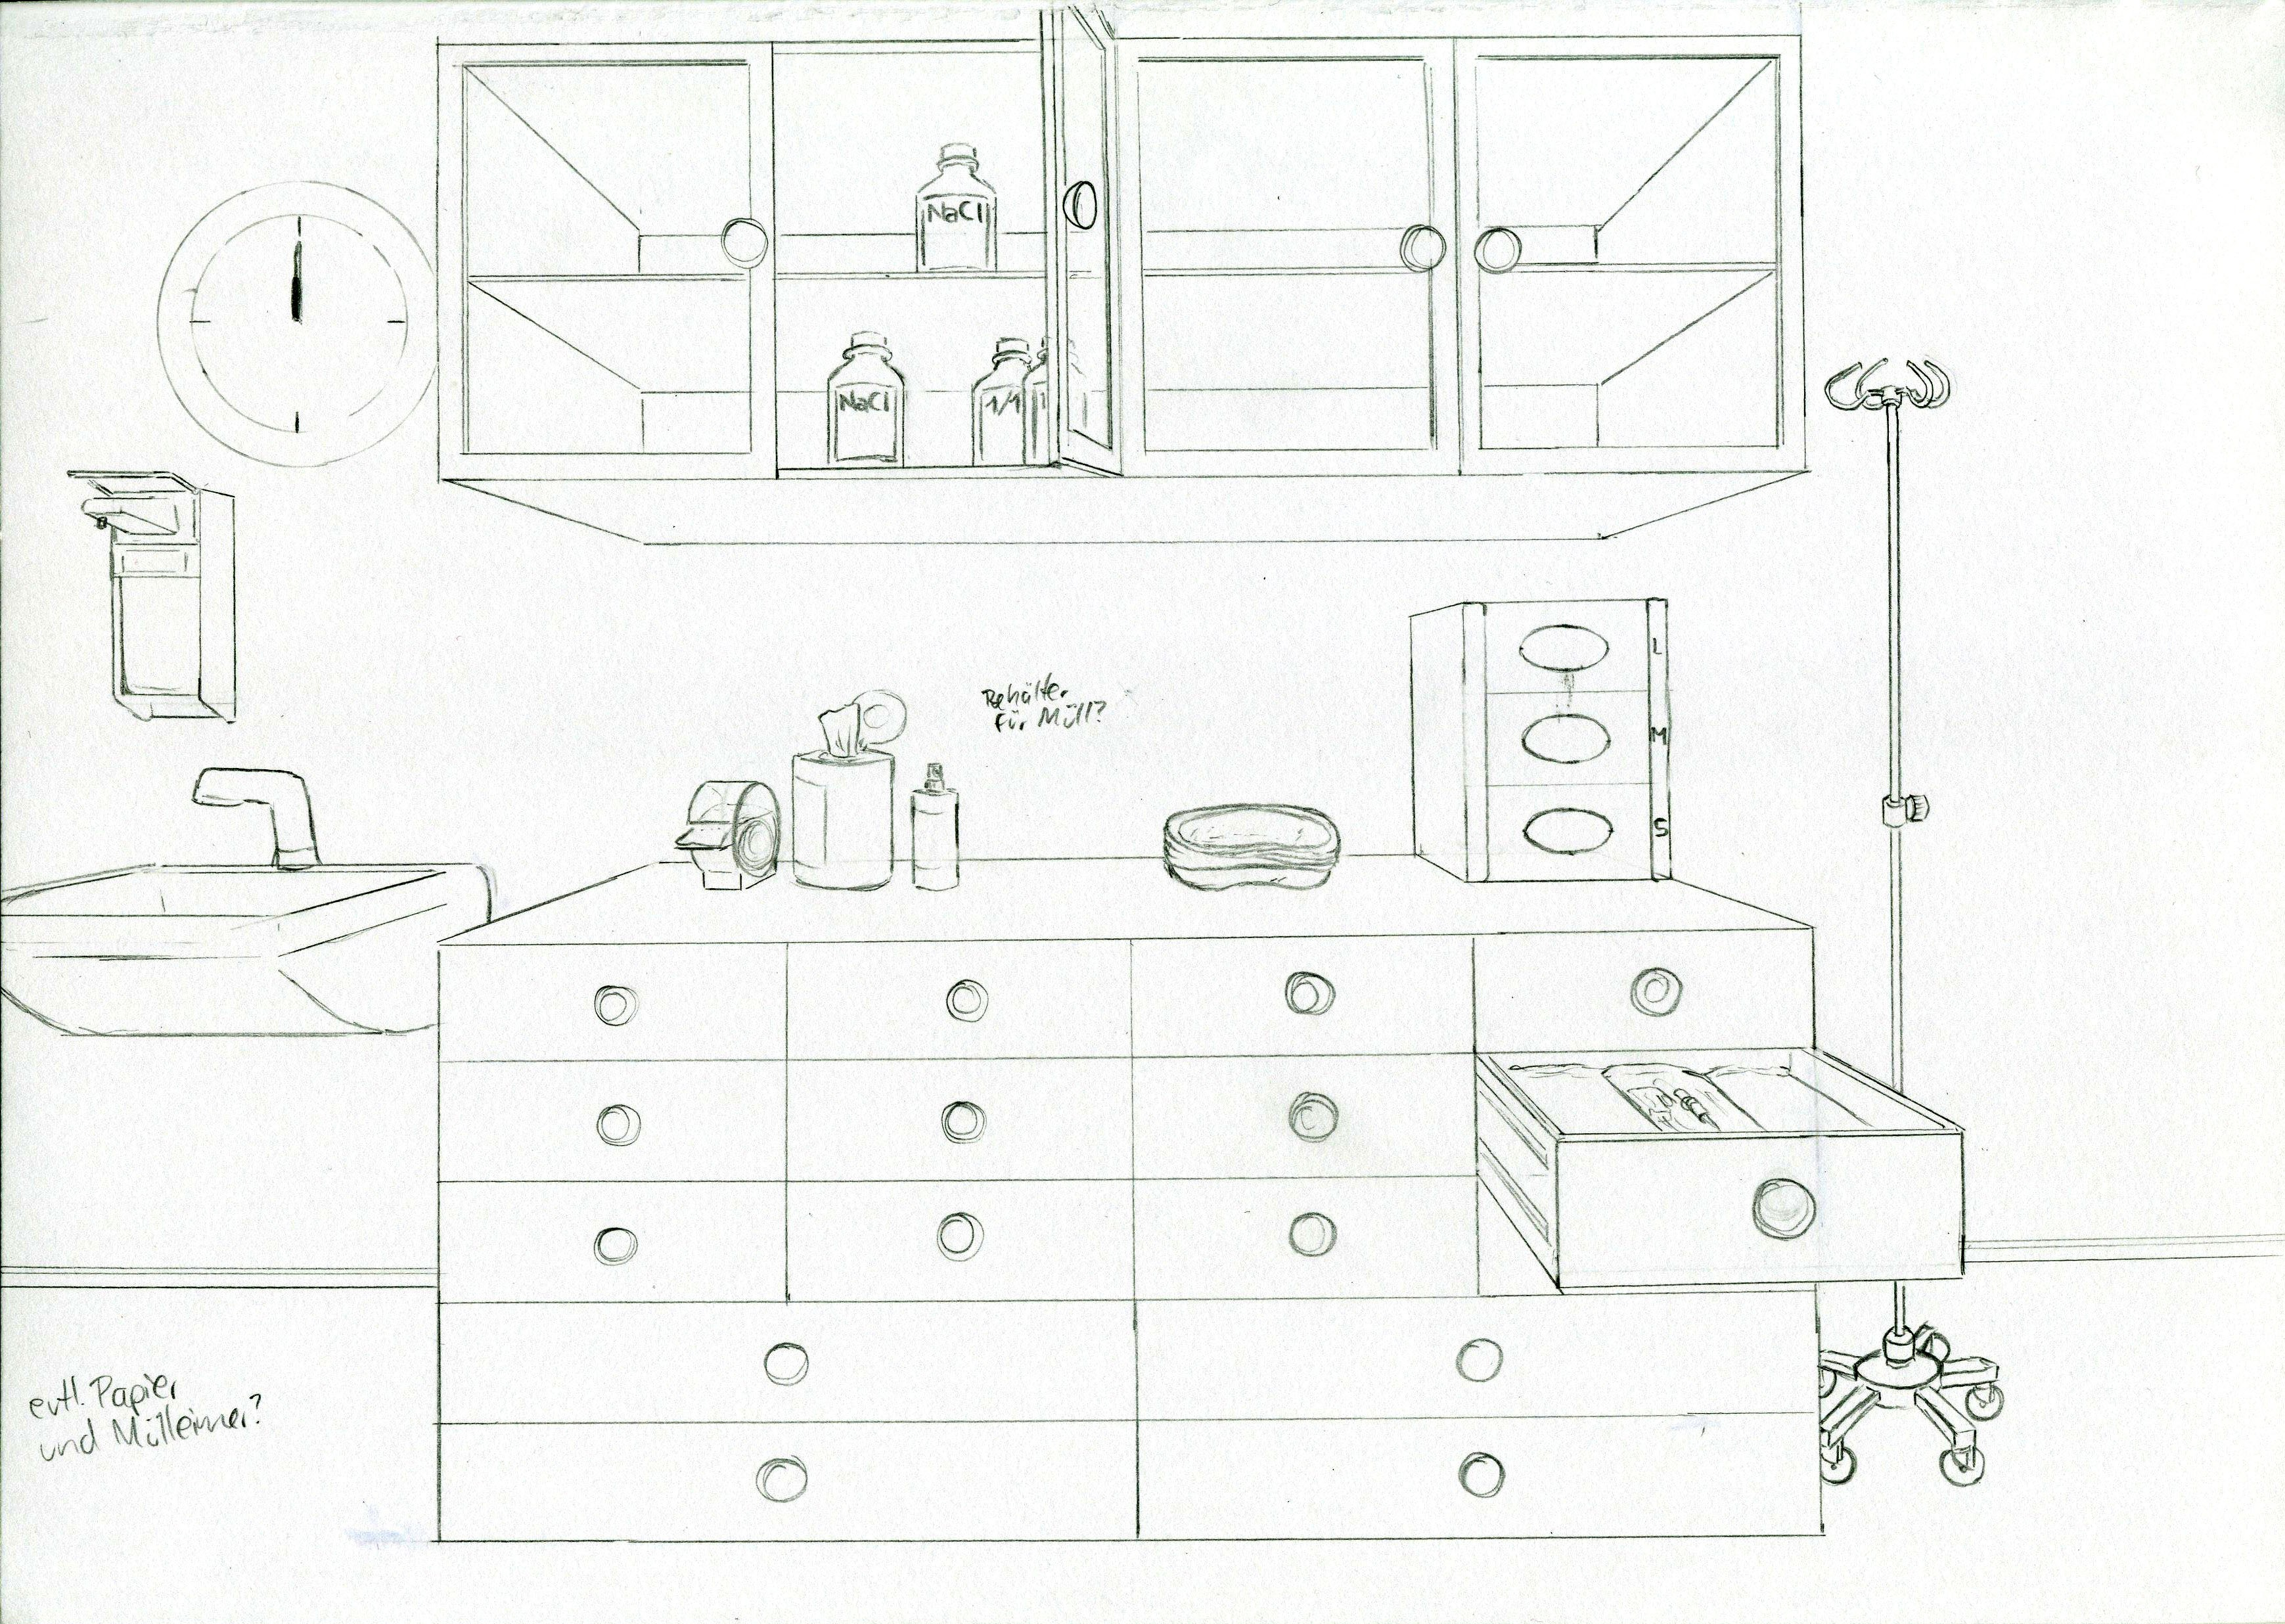
\includegraphics[width=\textwidth]{images/paperPrototype2.jpg}
  
  Der Aufbau der Szene basiert auf das Projekt, das im Jahr 2016 entwickelt wurde\citep{26}. Die Modells werden korrigiert und verbessert.
  
  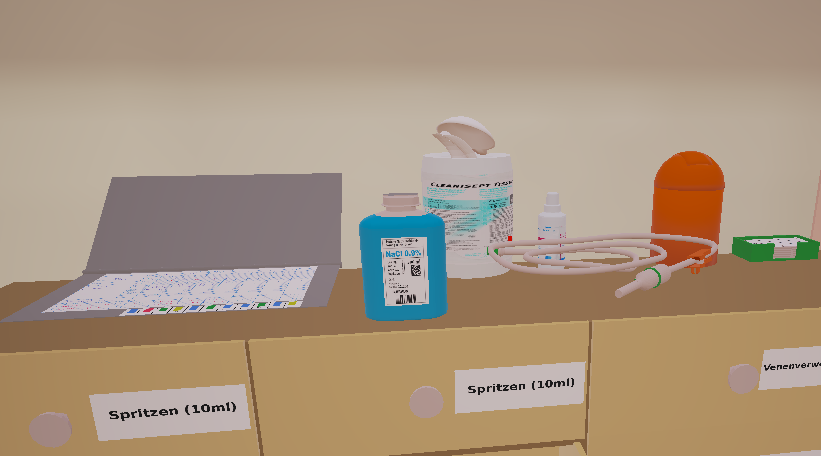
\includegraphics[width=\textwidth]{images/WithoutGlass.png}

   \subsubsection{lebendige Texturen}
   
   Um der Verbrauch der Leistung von Smartphone zu verringern, wurden unnötige Texturen damals nicht benutzt. Zurzeit besetzen Smartphone viel stärke Leistung, deshalb können die Modells mit lebendige Texturen gerendert werden, um das \glqq Vividness\grqq\ zu verbessern.
   
   Beispielsweise sind die wichtige Texturen:
   \begin{itemize}
       \item \textbf{Holz}: Hängeschränke, Schubladenschränke und Boden
       \item \textbf{Metal}: Griffen von Hängeschränke und Schubladenschränke, Handschuh-Dispenserhalter und Infusionsständer
       \item \textbf{farbiges Plastik}: Kanülen-Sammler,  Mülleimer, Spenderbox, Armhebelspender usw.
       \item \textbf{Wand}: Wände und Dach
   \end{itemize}
   
   \subsubsection{Transparenz}
   Die Objekte beispielsweise Infusionsflasche und Infusionsbesteck wurden im Jahr 2016 mit durchsichtige Materialien modelliert. Allerdings wurden die transparente Materialien nicht richtig in Gear VR dargestellt. Vermutlicher Grund war, dass die Leistung der damaligen Smartphones zu schwach war, weil die Renderung der transparenten Objekten sehr aufwendig ist.
   
   Im Jahr 2018 sind die Leistung der Smartphones schon viel stärker. Es soll möglich sein, in diesem Projekt die transparente Objekten zutreffend zu rendern.
   
   \subsubsection{Modell Korrektur von Kanülen-Sammler}
   Im Jahr 2016 wurde ein medizinischer Fehler bei der Modellierung gemacht, dass der Kanülen-Sammler mit normalen Mülleimer verwechselt wurde. Theoretisch ist Kanülen-Sammler schwierig zu öffnen, wenn der richtig zu gemacht. Im Gegenteil ist der Deckel des normalen Mülleimer sehr locker. Und es könnten die unsichere Situation passieren, dass der gebrauchte Spritze aus normalem Mülleimer ausfällt, wenn der Mülleimer eingesetzt würden.
   
\begin{figure}[ht]
\begin{minipage}[t]{0.48\linewidth}
\centering
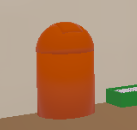
\includegraphics[width=\textwidth]{images/muelleimmer.png}
\caption[Skillslab WebVR]{Mülleimer}
\end{minipage}
\hspace{0.5cm}
\begin{minipage}[t]{0.48\linewidth}
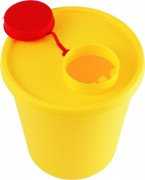
\includegraphics[width=\textwidth]{images/kanueleSammler.jpg}
\caption[Skillslab WebVR]{Kanülen-Sammler}
\end{minipage}
\end{figure}

In diesem Projekt wird den Fehler korrigiert.

   \subsubsection{Entfernung der Hinweis Streifen}
   Bei der 2016 Version wurde einen schwarzen Streife auf dem Boden der Sicht festgelegt, darauf die Hinweise und die Symbole Desinfektionstuch und Einmalhandschuhe gelegt wurden. Bei der Evaluation wurde das Problem getroffen, dass die Hinweise nicht angenehm gesehen könnten, weil es zu tief war. Jedoch könnte die Schwarze Streife nicht höher gesetzt werden, da würde zu viele Sicht versteckt.
   
   Um der schwarze Streif zu entfernen, werden erst die 3 zugehörige Aufgaben geteilt, und für jede Aufgabe eine andere Lösung finden.
   
   \begin{itemize}
       \item \textbf{Hinweise}: Die Aufgabe, Hinweise darzustellen wird von dem Whiteboard auf der links Seite des Raums übernommen.
       \item \textbf{Symbol von Desinfektionstuch}: Auf PC, Smartphone und Gear VR Version wird das Modell von dem Desinfektionstuch auf der Arbeitsfläche gelegt. Auf Vive Version kann das Desinfektionstuch direkt in Hand genommen werden. Deshalb ist das Symbol von Deinfektionstuch nicht nötig.
       \item \textbf{Symbol von Einmalhandschuhe}: Auf PC, Smartphone und Gear VR Version wird das Modell von Einmalhandschuhe direkt auf der Sicht hängt. Es bewegt sich nach der Bewegung der Kamera. Auf Vive Version wird die Modells von Händen mit Einmalhandschuhe mit der Farbe hell blau Dargestellt. Deswegen ist das Symbol von Einmalhandschuhe auch nicht mehr nötig. 
   \end{itemize}
   
   Mit diesen 3 Lösungen werden alle 3 zugehörigen Aufgaben übernommen, sodass kann der schwarze Streif entfernt werden.
   
   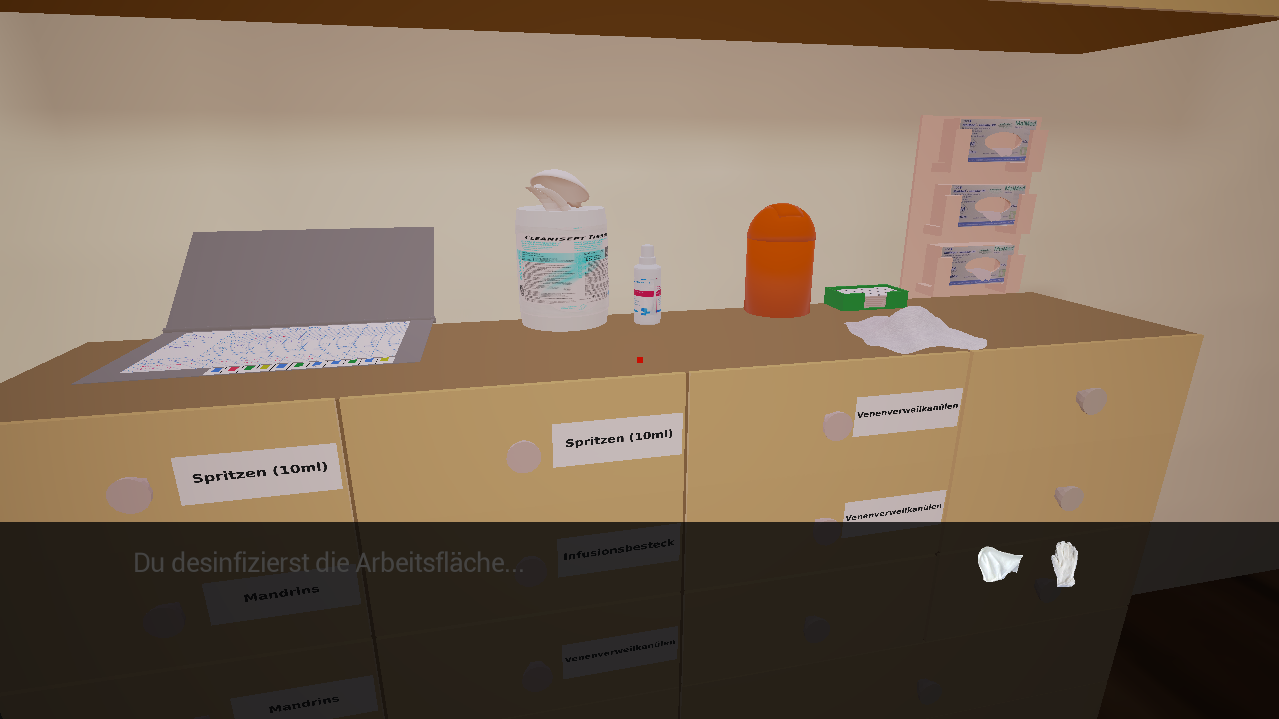
\includegraphics[width=\textwidth]{images/Schritt_4_2.png}

   \subsubsection{Modellierung für die Hände}
   Auf Vive Version können die Objekt durch den Controllers genommen und befreien. Die Controllers spielen die Rolle von Händen, deswegen sollen entsprechende Modells der Händen die Modells von Vive Controllers ersetzen.
   
   Die Modells der Händen sollen nach der Aktionen der Controllers animieren. Wenn der Auslöser gedrückt wird, soll die entsprechende Hand ein bisschen Faust machen. Im Gegenteil wenn der Auslöser freigegeben wird, soll die Faust befreit wird.


 \subsection{Interaktion}
 Interaktion ist ein wichtiger Teil der WebVR Applikation, weil die nicht nur die Implementierung von Interactability ist, sonder auch enge Beziehung mit Matching hat.
 
 Um bessere Benutzererfahrung zu haben, soll die Interaktionen auf der einen Seite die Merkmale der unterschiedlichen Geräte voll benutzen, auf der anderen Seite nicht zu vielfältig sein, sodass wird die Lernkosten erhöht. 
 
 Da die WebVr Applikation cross-platform ist, werden die Konzeptionen der Interaktion nach den Typen der Geräte gliedert.

 Für jede Geräte wird von drei Aspekten der Interaktionen erklärt:
 
 \textbf{Exploration}: Änderung der Aspekt.
 
 \textbf{Navigation}: Translation der Kamera.
 
 \textbf{Manipulation}: Aktivierung der Aktivität des Objektes für PC, Smartphone und Samsung Gear VR, zusätzlich Überprüfung, Greifen und Befreiung für HTC Vive.

 \subsubsection{PC}
 PC ist wichtiges Produktivitätswerkzeug für alle Leute. Im Vergleich mit Smartphone hat PC bessere Leistung und größer Bildschirm. Im Bereich E-Learning hat PC noch großer Vorteil bei Eingabe, deswegen spiele PC eine unersetzbare Rolle bei E-Learning. Durch WebVR Technik kann VR Umgebung in flachen Bildschirme gezeigt werden, damit wird die Erreichbarkeit der VR Applikation viel verbessert. 
 
  \textbf{Exploration}
  
  Um die VR Umgebung zu explorieren, wird den Aspekt verändert. Der Aspekt ist die Sicht, die in Kamera aufgenommen ist, nämlich die Sicht des Benutzers. Die Bewegung des Aspekts wird nach der Bewegung der Maus geführt. Es gibt zwei Varianten, um die Bewegung des Aspekts zu bestimmen.
  
  Eine Variante ist, dass die Bewegung des Aspekts aufgerufen wird, wenn die linke Taste der Maus gedrückt. Wenn die linke Taste losgelassen wird, bewegt sich der Aspekt nicht. Der Vorteil ist, dass solche Interaktion ähnlich wie alltägliche Applikation beispielsweise Google Map. Sodass wird die Interaktion schnell gewöhnt. Der Nachteil ist, dass eine Aktivität durch zwei Aktionen, Maus Druck und Maus Bewegung, aufgerufen werden. Das macht die Interaktion kompliziert, wenn der Aspekt sich häufig bewegt.
  
  Die andere Variante ist, dass die Bewegung Mode aktiviert wird. Das heißt, dass die Aspekt sich solange nach der Maus bewegt, bis ESC Taste gedrückt wird. Der Vorteil ist, dass die Interaktion einfach ist, und der Druck auf Maus verringert wird. Der Nachteil ist, dass der Mauszeiger während der Bewegung Mode verschwindet ist. Es könnte passiert, dass der Benutzer die Maus in einer großen Auswahl schwenkt, um den Mauszeiger zu finden, sodass der Aspekt auch schwer wackelt.
  
  Die verwirrende Aktivität bei zweite Variante passiert normalerweise nur bei der erst mal Nutzung und ist harmlos. Allerdings der Vorteil davon ist eindeutig. Deshalb wird die zweite Variante implementiert.
  
  \textbf{Navigation}
  
  Die Position der Kamera ist der Ort, wo der Benutzer in der VR Umgebung steht. Die Trandslation der Kamera führt zu die Navigation des Benutzers in dem simulierten Raum. Zwei Möglichkeiten der Navigation werden gebogen, eine zwingende und eine freiwillige.
  
  Zwingende Navigation bedeutet, dass die Kamera sich automatisch zu einem Ort bewegt, wenn die Translation die Benutzererfahrung verbessern kann. Das Ziel ist, der Benutzer zu leiten, Objekten zu betrachten. Zum Beispiel soll die Plakate über die Desinfektion der Hände Während der Desinfektion richtig betrachtet werden, deswegen bewegt sich die Kamera zwingend zu der Plakate, wenn der Benutzer Hände desinfizieren will.

  Außer der zwingende Bewegung kann die Kamera durch dem Druck auf den Tasten W, A, S, D navigieren. Das bietet die Freiheit, die VR Umgebung sich umzuschauen. Ohne die freiwillige Navigation kann die Übung auch barrierefrei durchgeführt werden.
  
  \textbf{Manipulation}
  
  Die Manipulation wird durch dem Zeiger durchgeführt. Zeiger ist ein schwarzer Ring, der immer in der Mittel der Sicht der Kamera steht. Der ist zuständig für den Aufruf eine Aktivität eines Objekts.
  
  Wenn der Benutzer mit dem nächsten Objekt hinter dem Zeiger interagieren kann, wechselt der Farbe des Rings zu grün, um das Selbstvertrauen dem Benutzer zu geben, die Aktivität zu aktivieren. Allerdings bedeutet der grüne Zeiger nicht, dass die Aktivität des Objekts aktiviert werden darf. Die Übung wird nach einer bestimmtem Reihenfolge durchgeführt, wenn eine Aktivität noch nicht daran ist, darf sie nicht aktiviert werden.
  
  Wenn der Zeiger grün ist und die linke Taste der Maus gedrückt wird, scheint die Farbe des Zeigers rot für ca. 0,3 Sekunde, und ein kurzes Soundeffekt geklungen wird, um die Botschaft an dem Benutzer geben, dass der Befehl, mit einem Objekt zu interagieren, ausgeführt ist. 
  
 \subsubsection{Smartphone}
 Laut der Forschung ist Mobile eine wichtige Trend von E-Learning. Ein wichtiger Faktor ist, dass die Mobilität des Smartphones unschlagbar ist. Smartphone bietet die Möglichkeit, in kurzem Zeitraum und im Verkehr zu lernen. Durch die WebVR Technik wird auch Smartphone unterstützt, VR Umgebung darzustellen.
 
  \textbf{Exploration}
  
  Zwei Methoden werden für Exploration angeboten, um unterschiedliche Situation anzupassen.
  
  Die intuitive Methode ist, das Smartphone zu bewegen. Der simulierte Umgebung wird in Smartphone räumlich dargestellt. Aber wegen die Begrenzung des Bildschirms ist nur den Raum teilweise im Blickwinkel. Durch die Bewegung des Smartphones wird andre Ort in dem Raum gesehen.
  

   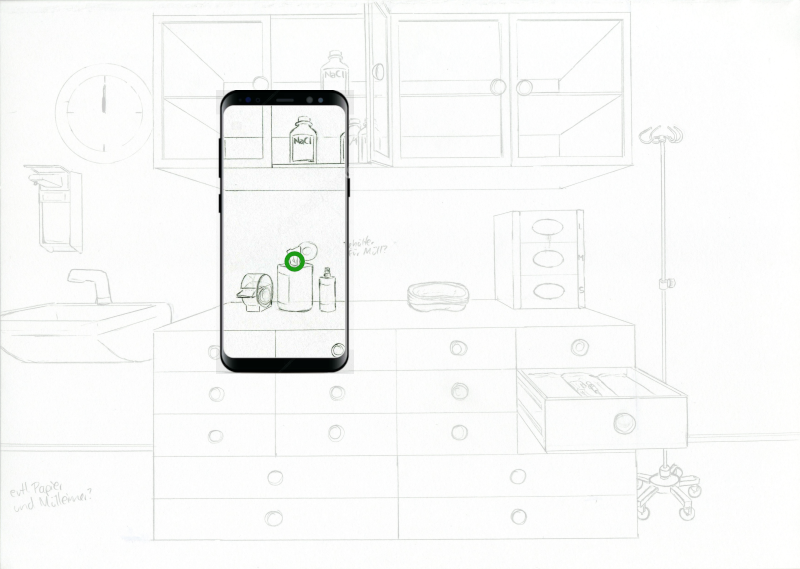
\includegraphics[width=\textwidth]{images/paperPrototypewiths8mini.png}

  
  Es ist unvermeidbar, den Körper zu drehen, um seitig gelegte Objekt zuzuschauen, wenn man mit der erste Methode das Smartphone bewegt. Allerdings ist es unmöglich, großer Winkel zu drehen, wenn man auf einem Stuhl sitzt. Außerdem beeinflusst es anderen Leute, wenn man in öffentlichem Raum beispielsweise Bibliothek große Bewegung macht. Um die Probleme zu lösen, wird die zweite Methode angeboten, dass der Aspekt durch dem Ziehen auf Bildschirm verändert wird. Obwohl diese Methode nicht so intuitive wie die erste Methode ist , vermehrt es sich die Einsatzmöglichkeiten.
  
  \textbf{Navigation}
  
  Das Smartphone bietet nur 3DoF Erkennung, nämlich Rotation. Deswegen kann die Translation des Kamera nicht mit der Translation des Smartphones verbinden. Um Objekt genauer anzuschauen und Interaktion zu vereinfacht, wird zwingend Navigation wie auf Laptop angeboten.
  
  \textbf{Manipulation}
  
  Der Form des Zeigers ist gleich wie auf Laptop. Da keine Maus zu Verfügung für Smartphone ist, wird die Bestätigung aus Zeiger durch \glqq Anstarr\grqq\ (eng. gaze) gesendet. Wenn der Zeiger vor einem Objekt ca. 0,5 Sekunde beliebt ist, wird es versucht, die Aktivität des Objeckts durchzuführen. Gleichzeitig wird ein kurz Soundeffekt geklungen.
  
 \subsubsection{Samsung Gear VR}
 Samsung Gear VR ist gut verbreitetes mobile HMD im Markt. Es ist ein typisch 3Dof HMD. Gear VR kann mit oder ohne Controller benutzt werden.
 
  \textbf{Exploration}
  
  Durch Gear VR wird der Benutzer in dem simulierten virtuellen Raum eingesetzt. Die Exploration wird durch der Rotation des Kopfs durchgeführt, ähnlich wie in reales Leben. Allerdings wird nur Rotation von HMD erkannt, weil Gear VR 3DoF ist.
  
  \textbf{Navigation}
  
  \textsl{Ohne Controller}: Wenn Gear VR ohne Controller ist, kann es Google Cupboard gelten. Die Navigation ist gleich wie die Navigation mit Smartphone, dass nur zwingend Navigation angeboten ist.
 
  \textsl{Mit Controller}: Der Gear VR Controller ist ein 3DoF Controller, dass nur die Rotation erkannt wird. Es soll eine Kurve aus dem Controller ausstrahlen, die auf dem Boden landen soll. Dort wird als der Zielort gezeichnet. Wenn den Tranlation Befehl durch dem Druck auf dem Trackpad auf dem Gear VR Controller gesendet, soll die Kamera sich zu dem gezeichnete Position navigiert.

  \textbf{Manipulation}
  
  \textsl{Ohne Controller}: Der Zeiger kann in zwei Formen möglich sein.
  
  Eine Möglichkeit ist, dass der Zeiger gleich wie auf Laptop und Smartphone als Ring gezeigt. Der Vorteil ist, dass der Zeiger eindeutig ist. Der Ring ist auf dem komplizierten Hintergrund (die Objekten in dem Raum) einfach zu kennen. Der Nachteil ist, dass der Treffpunkt mit Objekte nicht klar ist , besonders wenn das Ziel klein ist.
  
  Die andere Variante ist durch Raycaster. Raycaster ist eine von einer bestimmten Position ausstrahlende Linie, die die durchgegangene Objekte erkennen kann. In diesem Projekt wird das nächste Objekt zu dem Ausgangspunkt der Linie als das getroffene Objekt gezeichnet. Ein aus Augen Position ausstrahlendes Raycaster kann als der Zeiger gelten. Der Vorteil ist, dass die Position des Treffpunkts ganz genau ist. Der Nachteil ist, dass die Linie vor dem Komplizierten Hintergrund nicht auffallend ist.
  
  Die Merkmale der beiden Varianten sind eindeutig. Die Entscheidung für wird bei der Implementierung nach dem Endeffekt treffen.
  
  Die Bestätigung aus Zeiger kann durch dem Druck auf Touchpad von Gear VR oder auch durch \glqq Anstarr\grqq\ wie auf Smartphone durchgeführt werden. Als Feedback der Bestätigung wird ein kurz Soundeffekt geklungen. 
  
  \textsl{Mit Controller}: Ein Raycaster soll aus dem Controller ausstrahlen. Durch einem Druck auf dem Auslöser auf dem Controller wird es versucht, die Aktivität des getroffenen Objekt zu aktivieren. 
  
 \subsubsection{HTC Vive}
 HTC Vive ist ein 6DoF HMD mit starken Leistung. Es verbindet mit PC. Die WebVR Applikation kann durch normale Browser wie Firefox aufgerufen und die VR Umgebung wird gleichzeitig an dem HMD geschickt.
 
  \textbf{Exploration}
  
  Gleich wie mit Gear VR wird die Bewegung des Aspekts auch durch der Bewegung des Kopfs durchgeführt. Da HTC Vive 6DoF ist, werden nicht nur die Rotation sondern auch die Translation  erkannt. Sodass ist HTC Vive in der Lage, die Bewegung des Kopfs in der VR Umgebung völlig zu simulieren.
  
  \textbf{Navigation}
  
  Auch gleich wie mit Gear VR strahlt eine Kurve aus dem Controller, die auf dem Boden landet, und den Zielort zu bezeichnen. Durch dem Druck auf dem Trackpad auf dem Controller wird die Bewegung bestätigt und durchgeführt.
  
  \textbf{Manipulation}
  \begin{itemize}
  \item \textbf{Aktivierung der Aktivität des Objektes}: Durch dem Druck auf dem Auslöser wird es versucht, die Aktivität des Objektes zu aktivieren.
  \item \textbf{Greifen}: Wenn der Controller mit einem Objekt überlappt und der Auslöser auf dem Controller gedrückt und nicht befreit wird, wird das Objekt in dem Hand(Controller) gegriffen.
  \item \textbf{Befreiung}: Wenn ein Objekt in einem Hand(Controller) ist und deren Auslöser losgelöst wird, wird das Objekt befreit. Das heißt, dass das Objekt entweder auf eine bestimmte Position gelegt wird oder fällt.
  \item \textbf{Überprüfung}: Wenn ein Objekt überprüft werden muss, wird ein Raycaster aus der Position der Augen ausstrahlt. Wenn das Raycaster die richtige Position trifft und der Auslöser von einem leeren Hand gedrückt wird, wird die Überprüfung durchgeführt.
  \end{itemize}
  
  \begin{figure}[ht]
   \begin{minipage}[t]{0.48\linewidth}
   \centering
   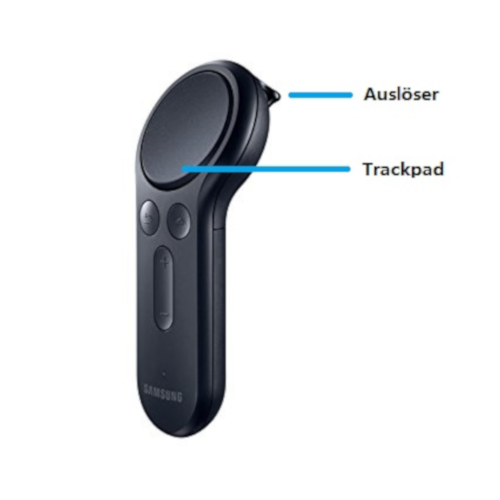
\includegraphics[width=\textwidth]{images/GearVRController.png}
   \caption[Skillslab WebVR]{Samsung Gear VR Controller}
   \end{minipage}
   \hspace{0.5cm}
   \begin{minipage}[t]{0.48\linewidth}
   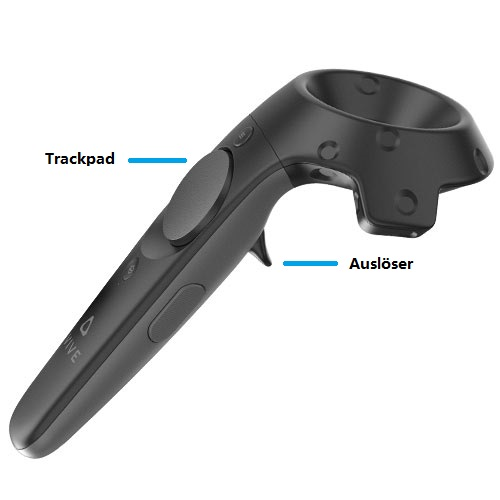
\includegraphics[width=\textwidth]{images/ViveController.jpg}
   \caption[Skillslab WebVR]{HTC Vive Controller}
   \end{minipage}
  \end{figure}
  
\begin{table}[]
\begin{tabular}{llll}
\hline
                                                                            & Exploration                                                                                                                                 & Navigation                                                                                                          & Manipulation                                                                                                                                                                                          \\ \hline
PC                                                                          & \begin{tabular}[c]{@{}l@{}}1.\\ Maus clicken\\ und bewegen\\ 2.\\ Maus clicken\\ dann bewegen\\ (ESC Tasten zu\\ deaktivieren)\end{tabular} & \begin{tabular}[c]{@{}l@{}}Frei:\\ W,A,S,D Tasten\\ \\ drücken\\ \\ Automaticsch:\\ Objekten anschauen\end{tabular} & \begin{tabular}[c]{@{}l@{}}Aktivieren:\\ Maus clicken\end{tabular}                                                                                                                                    \\ \hline
Smartphone                                                                  & \begin{tabular}[c]{@{}l@{}}1. Smartphone\\ bewegen\\ 2. Bildschirm\\ berühren\end{tabular}                                                  & \begin{tabular}[c]{@{}l@{}}Automatisch:\\ Objekt anschauen\end{tabular}                                             & \begin{tabular}[c]{@{}l@{}}Aktivieren:\\ Objekt anstarren\end{tabular}                                                                                                                                \\ \hline
\begin{tabular}[c]{@{}l@{}}Samsung\\ Gear VR\\ ohne Controller\end{tabular} & Kopf bewegen                                                                                                                                & \begin{tabular}[c]{@{}l@{}}Automatisch:\\ Objekt anschauen\end{tabular}                                             & \begin{tabular}[c]{@{}l@{}}Aktivieren:\\ 1.\\ Touchpack clicken\\ 2.\\ Objekt anstarren\end{tabular}                                                                                                  \\ \hline
\begin{tabular}[c]{@{}l@{}}Samsung\\ Gear VR\\ mit Controller\end{tabular}  & Kopf bewegen                                                                                                                                & Trackpad clicken                                                                                                    & \begin{tabular}[c]{@{}l@{}}Aktivieren:\\ Auslöser clicken\end{tabular}                                                                                                                                \\ \hline
HTC Vive                                                                    & Kopf bewegen                                                                                                                                & Trackpad clicken                                                                                                    & \begin{tabular}[c]{@{}l@{}}Aktivieren:\\ Auslöser clicken\\ \\ Greifen:\\ Auslöser drücken\\ \\ Befreien:\\ Auslöser loslösen\\ \\ Überprüfen:\\ Objekt anstarren\\ und Auslöser clicken\end{tabular} \\ \hline
\end{tabular}
\caption{Interaktionen unterschiedlichen Geräten}
\label{my-label}
\end{table}
  
 \subsection{Anordnung}
 Als eine Übung soll der Ablauf nach einer korrekten Reihenfolge durchgeführt werden. Um den korrekten und fließenden Ablauf zu garantieren, wird die VR Übung von drei Aspekten gestaltet, nämlich Planung des Ablaufs, Erkennung \& Feedback der Fortschritte und Leitung des Ablaufs. 
  \subsubsection{Planung des Ablaufs}
      
  Der Ablauf wird laut den fachlichen Anforderungen gestaltet. Insgesamt 23 Aktivität sollen während der Übung nach richtiger Reihenfolge gemacht werden. Die Aktivitäten werden unter acht Abschnitten unterteilt.
  
  \begin{enumerate}[start=0]
      \item Krankenakte überprüfen:
      
      Die Krankenakte wird von der Arbeitsfläche genommen. Die Informationen der Vorbereitung der Infusion werden laut 5R-Regel (richtiger Patient, richtiges Arzneimittel, richtige Dosierung, richtige Applikationsart, richtiger Zeitpunkt) überprüft. Danach wird die Krankenakte zurück gelegt.
      
      \item Hände desinfizieren:
      
      Die Hände werden 30 Sekunden desinfiziert.
      
      \item Arbeitsfläche desinfizieren:
      
      Einmalhandschuhe werden erst eingezogen. Danach wird Desinfektionstuch aus dem Dose ausgenommen. Schließlich wird die Arbeitsfläche desinfiziert. Die gebraucht Einmalhandschuhe und Desinfektionstuch werden in Mülleimer geworfen.
      \item Hände desinfizieren:
      
      Die Hände werden 30 Sekunden desinfiziert.
      
      \item Infusionsflasche vorbereiten:
      
      Die korrekte Flasche wird aus Schrank ausgenommen. Danach werden das Etikett, der Deckel und das Medikament überprüft. Am Ende wird die Flasche auf der Arbeitsfläche gelegt.
      
      \item Infusionsbesteck vorbereiten:
      
      Die Infusionsbesteck wird erst aus dem Schublade ausgenommen. Nach der Überprüfung der Etikett wird die Flasche auf der Arbeitsfläche gelegt und ausgepackt. Folglich wird die Durchflussregler zu und die Kappe des Dorns ab gemacht.
      
      \item Infusion vorbereiten:
      
      Nach der Abnahmen des Deckels der Flasche wird die Infusionsbesteck in der Flasche eingestrichen. Danach wird die Flasche auf dem Infusionsständer gehängt. Durch dem Druck auf dem Tropfkammer lässt die Medikament im Tropfkammer tropfen. Durch die Öffnung der Durchflussregler wird die transparenten Infusionsleitung mit Medikament ausgefüllt. Am Ende wird die Infusionsleitung festgelegt.
      
      \item Namenetikett vorbereiten:
      
      Nach der Ausfüllung wird eine Namenetikett auf der Flasche geklebt.
      
  \end{enumerate}
      
  \begin{figure}[ht]
  \begin{minipage}[t]{1\linewidth}
  \centering
  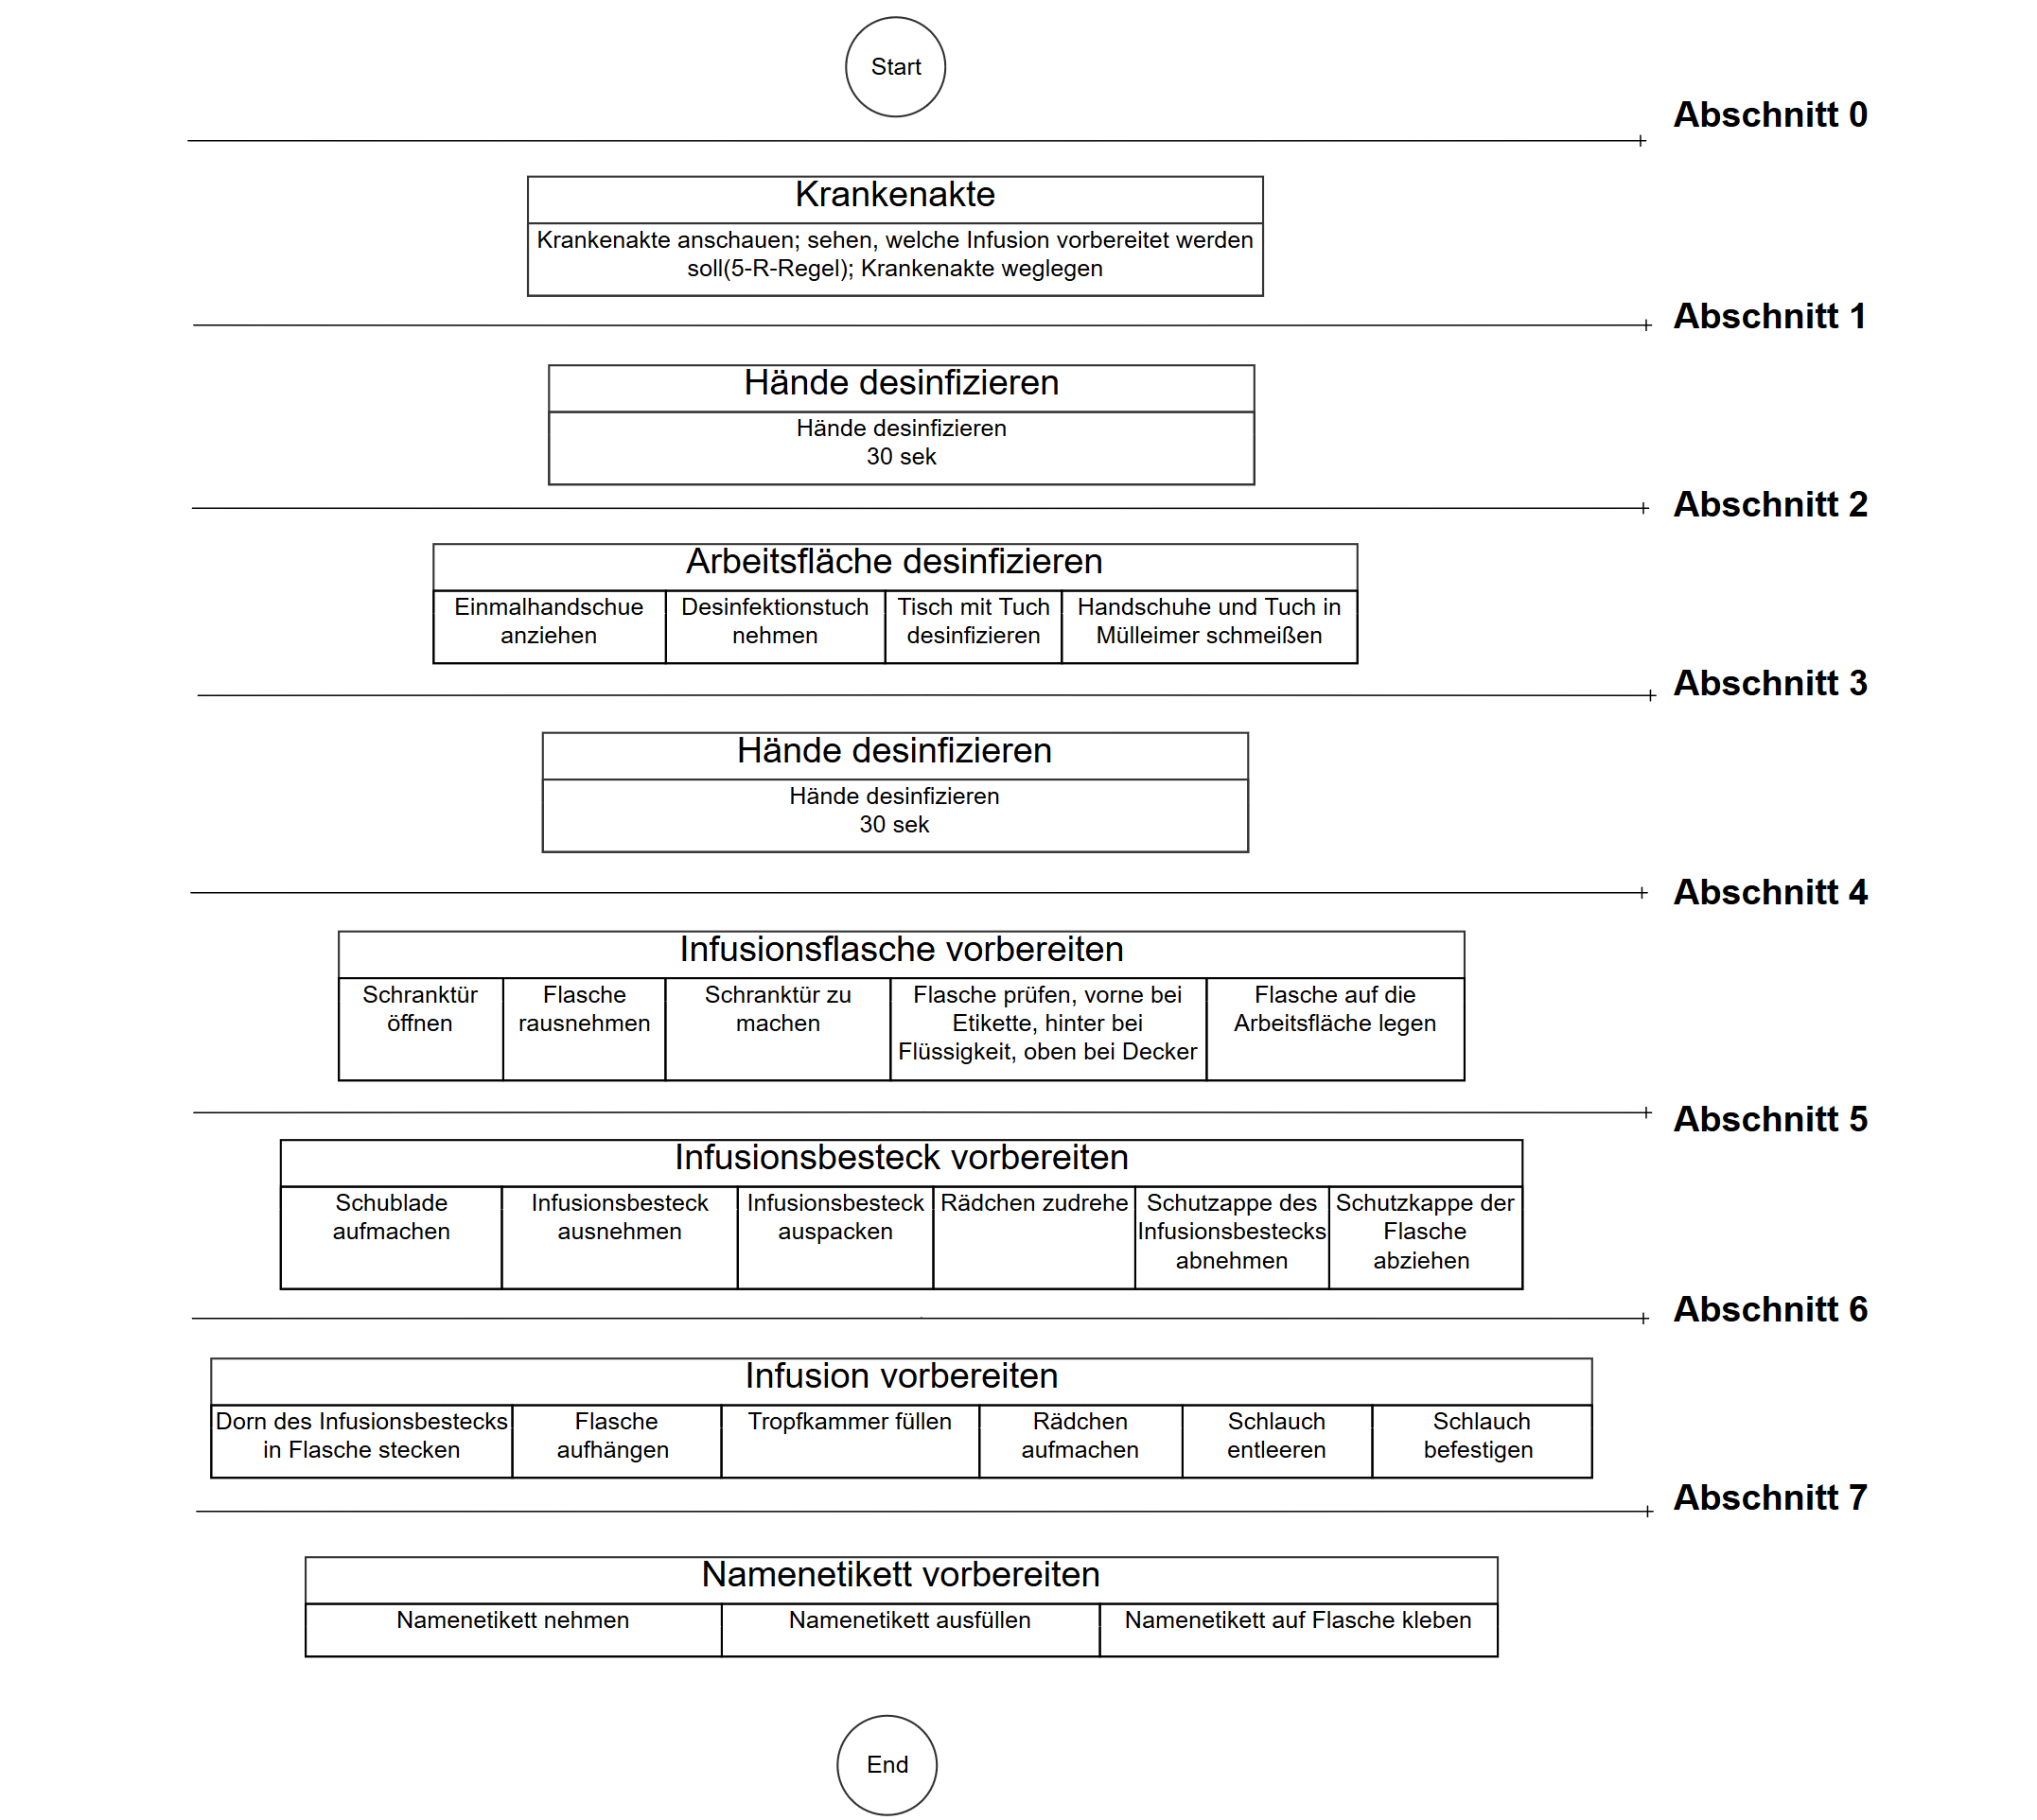
\includegraphics[width=\textwidth]{images/infusion_vorbereitung_durchlauf.png}
  \caption[Skillslab WebVR]{Ablauf}
  \end{minipage}
  \end{figure}
  
  Die Abschnitte sind nicht nur die abstrakte Gliederung, sondern auch die Optionen, damit für die erste Aktivität in der Übung entschieden werden kann. Der Auswahl des Abschnitts kann entweder in der VR Umgebung oder bei dem Unterricht in LMS getroffen werden.
  
  \subsubsection{Erkennung \& Feedback der Fortschritte}
  Der Fortschritt des Prozesses der Übung wird durch der Durchführung einer richtigen Aktivität gefördert. Wenn eine Aktivität des Objektes zur richtigen Zeit durchgeführt wird, wird der Fortschritt erkannt. Die Erkennungen müssen durch den oben genannten Interaktionen nämlich Manipulationen der VR Geräten bewältigt wird.
  
  Auf PC, Smartphone und Gear VR führt eine wirksame Manipulation zu einem Schritt vor. Allerdings für HTC Vive ist es nicht gleich, weil die 6 DoF Geräten mehr Freiheit der Interaktion besetzen. Zum Beispiel fördert die Abholung eines gefallenen Objektes den Prozess der Übung nicht. 
  
  Die Feedbacks der Fortschritt bieten den Bescheid, dass die aktuelle Aufgabe erledigt wird, die nächste Aufgabe gemacht werden soll. Die Feedbacks werden meistens im Form Animation (Translation und Rotation) des Objektes gegeben. Außerdem können die Feedbacks durch die Änderung der Eigenschaft(Sichtbarkeit, Farbe) gegeben werden. Zum Beispiel wird ein Haken dargestellt, wenn das Name von Patient überprüft wird.
  
  \subsubsection{Leitung des Ablaufs}
  Der Fortschritt wird durch die richtigen Aktivitäten durchgeführt. Die Versuche, mit dem richtigen Objekt im falschen Zeitraum oder mit den falschen Objekten zu interagieren, werden ignoriert. Um der Prozess der Übung zu leiten, wird vier Hilfsmitteln angeboten, nämlich Whiteboard, Hilfe-Box, 30 Sekunden Indikator und Hacken.
  \begin{itemize}
      \item \textbf{Whiteboard}:
      
      Ein Whiteboard wird auf dem linken Wand gehängt, um die Hinweise anzubieten. Wenn eine Aufgabe geschafft wird, wird der Hinweis für nächsten Aufgabe auf dem Whiteboard gezeigt. Wenn der Benutzer an dem nächsten Schritt nicht erinnern kann, kann er den Kopf nach links drehen, um die Hinweis zu lesen.
      
      Während der Übung führt keine Aufgabe außer Händedesinfektion zur der Drehung des Kopfs nach links. Das heißt, obwohl der Hinweis dargestellt ist, kann der Benutzer den Hinweis nur durch die absichtliche Drehung des Kopfs nach links lesen. Somit wird die unabsichtliche Vorsagen vermeidet.
      
      \item \textbf{Hilfe-Box}:
      
      Hilfe-Box ist ein halbe transprenter Kasten, die in der VR Umgebung dargestellt ist, wenn ein Objekt in Hand ist. Hilfe-Box hat zwei Funktionalitäten. Eine davon ist, die Position zu bezeichnen, wohin das Objekt gelegt werden soll. Die andere Funktionalität ist, die Zustände des genommenen Objektes zu zeigen. Wenn ein Objekt gerade in Hand genommen wird, wird das Hilfe-Box dafür in Rot dargestellt. Wenn alle Aufgabe, z.B Überprüfung, zu diesem Objekt erledigt werden,  wird die Farbe des Objektes zu Grün gewechselt, um dem Benutzer zu informieren, darf das Objekt hingelegt werden. Wenn das Objekt in dem entsprechenden Hilfe-Box hingelegt, verschwindet das Hilf-Box und wir die Position des Objektes angepasst.
      
      \item \textbf{30 Sekunden Indikator}:
      
      Laut fachliche Anforderung soll die händedesinfektion 30 Sekunden dauern. Um eine eindeutige Zeichnung, die genaue Zeit darzustellen, wird eine Uhr über dem Armhebelspender für Händedesinfektionsmittel gehängt. Die Uhrzeit darauf ist genau wie die Zeit in realem Welt.
      
      Der 30 Sekunden Indikator ist ein roter Halbkreis auf der Platte der Uhr, der genau 30 Sekunden bezeichnet. Wenn der Griff des Armhebelspender gedruckt wird, erscheint der 30 Sekunden Indikator, deren Ausgangsposition auf dem Sekundenzeiger liegt.
      
      Wenn 30 Sekunden abgelaufen, verschwindet der 30 Sekunden Indikator, um dem Benutzter zu informieren, dass die Händedesinfktion fertig ist und weitere Aufgaben behandeln dürfen.
      
      \item \textbf{Hacken}:
      
      Hacken bezeichnet die gecheckt Element, zum Beispiele 5-R bei Überprüfung der Krankenakte.
  \end{itemize}
  
\begin{table}[]
\resizebox{\textwidth}{!}{%
\begin{tabular}{llll}
\hline
            & Position                                                                         & rot                                                                                                      & grün                                                                                                     \\ \hline
Abschnitt 0 & \begin{tabular}[c]{@{}l@{}}Obere linke\\ Ecke der Arbeitsoberfläche\end{tabular} & Krankenakte in Hand                                                                                      & 5R überprüft                                                                                             \\ \hline
Abschnitt 2 & Über dem Mülleimer                                                               & Desinfektionstuch in Hand                                                                                & Arbeitsoberfläche desinfiziert                                                                           \\ \hline
Abschnitt 4 & Auf der Arbeitsoberfläche                                                        & Infusionsflasche in Hand                                                                                 & Infusionsflasche überprüft                                                                               \\ \hline
Abschnitt 5 & Auf der Arbeitsoberfläche                                                        & Infusionsbesteck in Hand                                                                                 & Infusionsbesteck überprüft                                                                               \\ \hline
Abschnitt 6 & \begin{tabular}[c]{@{}l@{}}Unter dem Hacken\\ der Infusion Stand\end{tabular}    & \begin{tabular}[c]{@{}l@{}}Infusionsflasche mit\\ eingestochenem Infusionsbesteck\\ in Hand\end{tabular} & \begin{tabular}[c]{@{}l@{}}Infusionsflasche mit\\ eingestochenem Infusionsbesteck\\ in Hand\end{tabular} \\ \hline
Abschnitt 7 & Auf der Infusionsflasche                                                         & Namenetikett in Hand                                                                                     & Nameneitkett ausgefüllt                                                                                  \\ \hline
\end{tabular}%
}
\caption{Nutzung der Hilfe-Boxes}
\label{my-label}
\end{table}

  
\subsection{Zusammenfassung}
Web basierte Applikation wie LMS ist weit verbreitet. Browser kann aus der Sicht der Anwendung sogar als mini-Betriebssystem gelten. Deshalb besetzt die Web VR Applikation einen unersetzbaren Vorteil, barrierefrei mit andere web basierte Applikation zu integrieren.

Als eine Anwendung einer cross-platform Technik müssen der Entwickler während der Konzeption mit unterschiedlichen Geräten rechnen, um bessere Erreichbarkeit zu realisieren.

Das immersive Erlebnis kann lebendige Umgebung und mehr interaktive Aktivitäten anbieten. Allerdings soll das VR-Training die richtige und fachliche Kenntnisse vermitteln, deswegen wird die interaktive Freiheiten in diesem Projekt begrenzt.

Durch die Verbindung zwischen E-Learning und VR-Training werden die Nachteile von den beiden überwunden. Theoretisch soll die neue Lernmethode effektive sein.
  
  \subsubsection{Abschnitte}
  
  \subsubsection{White board}
  
  \subsubsection{Hacken}
  
  \subsubsection{Hilfe Boxes}
  
  \subsubsection{Zustand des Ablaufs in Implementierung}
  
\begin{itemize}
\item UI
\item white board
\item Interaktion
\subitem flach Bildschirm: cursor, gaze
\subitem GearVR: gaze, click
\subitem HTC Vive: drag, press release, hand, check
\subitem observer patern---------
\item Töne
\item section selection: observerpatern------
\item hand
\item collision
\item check 3 Dingen
\end{itemize}